\chapter{L'intensité du courant et l'ampèremètre}\label{ch:g8:intensity-ammeter}

«~Courant fort, courant faible~» --- nous parlons ainsi depuis des
années, en dosant l'éclat et la prise au jugé. Le jugé prend sa
retraite aujourd'hui. L'\omterm{def:g8:intensity-ammeter:intensity}{intensité} du courant reçoit un nom, une \omterm{def:g6:measurement-in-science:measuring}{unité}
et un instrument~; et la première chose que l'instrument démontre est
une loi que tu soupçonnais depuis longtemps sans l'avoir jamais
mesurée.

\section{L'intensité et son unité}

\begin{definition}[Intensité]\label{def:g8:intensity-ammeter:intensity}
L'\emph{intensité}\index{intensité} $I$ d'un \omterm{def:g7:circuits-series-parallel:current}{courant électrique}
mesure la vigueur de la marche~: quelle quantité de charge électrique
défile par seconde devant un point du circuit --- le débit du
courant, comme celui d'une rivière est une quantité d'eau par
seconde. Son \omterm{def:g6:measurement-in-science:measuring}{unité} est l'\emph{ampère}\index{ampère} (\unit{A}), en
l'honneur d'un grand pionnier des lois de l'électricité~; les
circuits de tous les jours parlent souvent en
\emph{milliampères}~: $\qty{1}{mA} = \qty{0.001}{A}$, un
millième.
\end{definition}

\begin{example}[Des ampères à reconnaître d'un coup
d'œil]\label{ex:g8:intensity-ammeter:values}
Un petit voyant lumineux sirote environ \qty{0.02}{A} ---
\qty{20}{mA}~; une ampoule de lampe de poche, autour de
\qty{0.3}{A}~; le gros phare d'une voiture, \qty{5}{A}~; une
bouilloire à plein régime, \qty{10}{A}~; un moteur de voiture qui
démarre avale \qty{100}{A} à sa batterie~; un éclair, le temps de sa
milliseconde, enfonce des dizaines de milliers d'\omterm{def:g8:intensity-ammeter:intensity}{ampères} dans son
canal. Et l'échelle du danger donne à réfléchir~: des courants de
quelques centièmes d'\omterm{def:g8:intensity-ammeter:intensity}{ampère} à travers un corps humain peuvent déjà
être mortels --- le respect commence bien au-dessous d'un \omterm{def:g8:intensity-ammeter:intensity}{ampère}.
\end{example}

\begin{remark}[La personne et l'unité]\label{rem:g8:intensity-ammeter:person}
Écrite en toutes lettres, l'\omterm{def:g6:measurement-in-science:measuring}{unité} prend une minuscule --- «~un
courant de deux \omterm{def:g8:intensity-ammeter:intensity}{ampères}~» --- tandis que le mot avec majuscule nomme
la personne, comme pour toute \omterm{def:g6:measurement-in-science:measuring}{unité} qui honore un savant. Le symbole
\unit{A}, lui, reste en capitale. Tu retrouveras bientôt cette
convention, deux fois.
\end{remark}

\section{L'ampèremètre}

\begin{definition}[Ampèremètre]\label{def:g8:intensity-ammeter:ammeter}
Un \emph{ampèremètre}\index{ampèremètre} mesure l'\omterm{def:g8:intensity-ammeter:intensity}{intensité}. Il
compte la marche qui passe \emph{à travers lui} --- il doit donc être
inséré \emph{\omterm{def:g4:series-circuits:series}{en série}}, dans la boucle même qu'il mesure, comme un
péage sur la route. Construit pour déranger la marche aussi peu que
possible, il ne s'oppose presque pas au courant --- et c'est aussi
pourquoi un ampèremètre branché par erreur directement en travers
d'une \omterm{def:g3:first-electric-circuit:battery}{pile} est un \omterm{def:g7:short-circuits-safety:device}{court-circuit} muni d'un cadran~: la façon classique
d'en casser un.
\end{definition}

\begin{method}[Mesurer une intensité]\label{met:g8:intensity-ammeter:measure}
\begin{enumerate}
  \item couper le circuit~; \emph{ouvrir} la boucle à l'endroit où
        le courant doit être compté~;
  \item insérer l'\omterm{def:g8:intensity-ammeter:ammeter}{ampèremètre} dans la coupure~: le courant entre
        par sa \omterm{def:g3:first-electric-circuit:battery}{borne} \unit{A} et ressort par sa \omterm{def:g3:first-electric-circuit:battery}{borne}
        \emph{commune}, de sorte que le sens conventionnel entre
        par la porte d'entrée de l'appareil~;
  \item sur un appareil à plusieurs calibres, commencer par le
        \emph{plus grand} calibre, puis descendre jusqu'à ce que la
        lecture s'installe confortablement sur le cadran --- ce qui
        protège l'appareil des surprises~;
  \item fermer l'\omterm{ex:g3:first-electric-circuit:switch}{interrupteur}, lire --- et écrire l'\omterm{def:g6:measurement-in-science:measuring}{unité}.
\end{enumerate}
Un branchement à l'envers sur un appareil à aiguille projette celle-ci
contre sa butée~; les appareils numériques se contentent d'afficher un
signe moins, et pardonnent aux élèves tous les jours.
\end{method}

\begin{omfigure}
\begin{tikzpicture}[scale=0.9]
  \draw (0,0) to[battery1, l=pile] (0,2.8)
    to[short] (1.8,2.8)
    to[ammeter, l=$I$] (4.2,2.8)
    to[lamp, l=lampe] (6.6,2.8)
    to[short] (8.0,2.8)
    to[short] (8.0,0)
    to[short] (0,0);
  \draw[-Stealth, very thick, omThm] (1.0,3.15) -- (1.7,3.15);
\end{tikzpicture}

{\small L'\omterm{def:g8:intensity-ammeter:ammeter}{ampèremètre} prend sa place dans la boucle~: un péage \omterm{def:g4:series-circuits:series}{en
série}, qui compte la marche allumant la lampe.}
\end{omfigure}

\begin{omfigure}
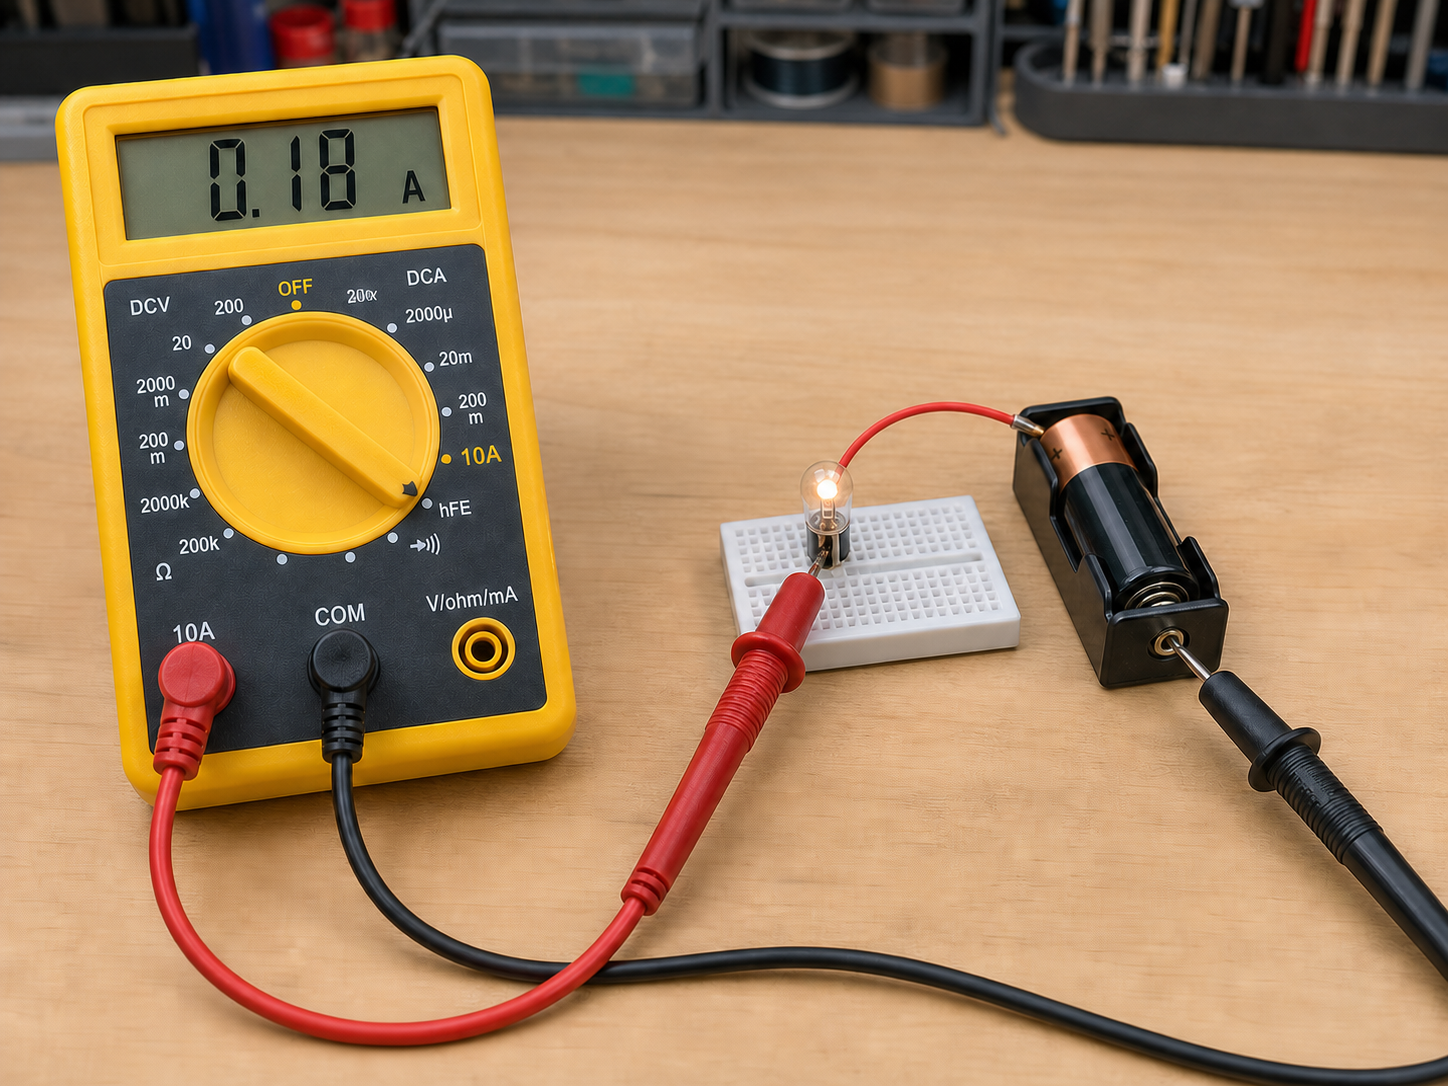
\includegraphics[width=0.5\linewidth]{images/book1/ai/g8-ammeter-multimeter.png}

{\small La réalité de l'établi~: un appareil, deux pointes de touche, et le courant du circuit devient un nombre sur l'afficheur.}
\end{omfigure}

\section{La première loi mesurée}

\begin{proposition}[Une boucle, une intensité]\label{prop:g8:intensity-ammeter:sameI}
Dans un \omterm{def:g4:series-circuits:series}{circuit en série}, l'\omterm{def:g8:intensity-ammeter:intensity}{intensité} est la même en tout point de la
boucle. Déplace l'\omterm{def:g8:intensity-ammeter:ammeter}{ampèremètre} où tu veux --- avant la lampe, après
elle, à côté de la \omterm{def:g3:first-electric-circuit:battery}{pile}~: la lecture ne change pas. Ce que cinq
années de lampes d'éclat égal suggéraient, l'appareil l'énonce
maintenant en nombres~: rien n'est consommé en route~; une route, une
marche, un seul $I$.
\end{proposition}

\begin{omfigure}
\begin{tikzpicture}[scale=0.85]
  \draw (0,0) to[battery1] (0,3.0)
    to[ammeter, l=\qty{0.30}{A}] (2.6,3.0)
    to[lamp] (4.8,3.0)
    to[ammeter, l=\qty{0.30}{A}] (7.4,3.0)
    to[lamp] (9.6,3.0)
    to[short] (9.6,0)
    to[ammeter, l=\qty{0.30}{A}] (4.8,0)
    to[short] (0,0);
\end{tikzpicture}

{\small Trois péages sur une seule boucle~: avant, entre et après les
lampes, chaque \omterm{def:g8:intensity-ammeter:ammeter}{ampèremètre} annonce les mêmes \qty{0.30}{A}.}
\end{omfigure}

\begin{example}[Lire les petites lignes de la
loi]\label{ex:g8:intensity-ammeter:fineprint}
La loi dit \emph{le long d'une même boucle}, non \emph{quoi que tu
fasses à la boucle}. Ajoute une seconde lampe \omterm{def:g4:series-circuits:series}{en série} et la marche
faiblit partout à la fois --- peut-être les \qty{0.30}{A}
tombent-ils à \qty{0.17}{A} --- mais elle faiblit \emph{également}
partout~: les trois péages s'accordent aussi sur le nouveau nombre.
Une boucle, une \omterm{def:g8:intensity-ammeter:intensity}{intensité} --- quelle que soit cette \omterm{def:g8:intensity-ammeter:intensity}{intensité} du
moment.
\end{example}

\begin{example}[Un coup d'œil au nœud]\label{ex:g8:intensity-ammeter:junction}
Installe plutôt des péages sur une paire \omterm{def:g5:series-parallel-circuits:parallel}{en dérivation}~: route
principale \qty{0.50}{A}~; \omterm{def:g5:series-parallel-circuits:parallel}{branche} numéro un \qty{0.30}{A}~; \omterm{def:g5:series-parallel-circuits:parallel}{branche}
numéro deux \qty{0.20}{A}. La somme suggestive n'est pas un hasard
--- les marches qui entrent dans un \omterm{def:g5:series-parallel-circuits:parallel}{nœud} et celles qui en sortent
doivent s'équilibrer, puisque la charge n'est ni créée ni détruite à
un embranchement. La loi complète, avec sa partenaire pour la
tension, tiendra séance dans deux chapitres~; tes appareils l'ont
déjà rencontrée.
\end{example}

\begin{remark}[Le multimètre]\label{rem:g8:intensity-ammeter:multimeter}
La brique jaune de l'atelier --- le \emph{multimètre} --- replie
l'\omterm{def:g8:intensity-ammeter:ammeter}{ampèremètre} et plusieurs autres instruments dans un seul boîtier
muni d'un sélecteur. Sélecteur sur \unit{A} ou \unit{mA}, cordons
dans les prises marquées, et c'est ton \omterm{def:g8:intensity-ammeter:ammeter}{ampèremètre}, règles de la
série comprises. Deux chapitres de ce livre habitent déjà à
l'intérieur~; un troisième y emménage au chapitre suivant --- avec,
attention, des règles de branchement \emph{opposées}.
\end{remark}

\section{Exercices}

\begin{exercise}[$\star$]\label{exo:g8:intensity-ammeter:1}
Que mesure l'\omterm{def:g8:intensity-ammeter:intensity}{intensité}, en langage de rivière~? Donne son \omterm{def:g6:measurement-in-science:measuring}{unité} et
son symbole, et convertis \qty{250}{mA} en \omterm{def:g8:intensity-ammeter:intensity}{ampères}.
\end{exercise}

\begin{exercise}[$\star$]\label{exo:g8:intensity-ammeter:2}
Associe l'\omterm{def:g8:intensity-ammeter:intensity}{intensité} à sa scène~: \qty{0.02}{A}~; \ \qty{0.3}{A}~; \
\qty{10}{A}~; \ \qty{100}{A} --- bouilloire, voyant lumineux, \omterm{ex:g6:circuits-and-safety:motor}{moteur}
qui démarre, ampoule de lampe de poche.
\end{exercise}

\begin{exercise}[$\star$]\label{exo:g8:intensity-ammeter:3}
Pourquoi un \omterm{def:g8:intensity-ammeter:ammeter}{ampèremètre} doit-il être inséré \omterm{def:g4:series-circuits:series}{en série}~? À quoi
est-il construit pour ne presque pas s'opposer, et quel accident cela
rend-il possible~?
\end{exercise}

\begin{exercise}[$\star$]\label{exo:g8:intensity-ammeter:4}
Énumère les quatre étapes d'une mesure d'\omterm{def:g8:intensity-ammeter:intensity}{intensité} bien faite.
Pourquoi commencer par le plus grand calibre~?
\end{exercise}

\begin{exercise}[$\star$]\label{exo:g8:intensity-ammeter:5}
Énonce la loi «~une boucle, une \omterm{def:g8:intensity-ammeter:intensity}{intensité}~». Quelle vieille
observation d'éclats égaux a-t-elle transformée en nombres~?
\end{exercise}

\begin{exercise}[$\star$]\label{exo:g8:intensity-ammeter:6}
Un \omterm{def:g8:intensity-ammeter:ammeter}{ampèremètre} placé avant un \omterm{ex:g6:circuits-and-safety:motor}{moteur} \omterm{def:g4:series-circuits:series}{en série} indique \qty{0.45}{A}.
Qu'indiquera-t-il après le \omterm{ex:g6:circuits-and-safety:motor}{moteur}~? Et à côté de la \omterm{def:g3:first-electric-circuit:battery}{pile}~?
\end{exercise}

\begin{exercise}[$\star$]\label{exo:g8:intensity-ammeter:7}
Une seconde lampe rejoint une boucle \omterm{def:g4:series-circuits:series}{en série} et les \qty{0.30}{A} de
l'\omterm{def:g8:intensity-ammeter:ammeter}{ampèremètre} deviennent \qty{0.17}{A}. La loi est-elle en défaut~?
Explique les petites lignes.
\end{exercise}

\begin{exercise}[$\star$]\label{exo:g8:intensity-ammeter:8}
Un \omterm{def:g8:intensity-ammeter:ammeter}{ampèremètre} numérique indique $-0.25$ \unit{A}. Qu'a fait
l'élève, et quelle est la gravité~?
\end{exercise}

\begin{exercise}[$\star\star$]\label{exo:g8:intensity-ammeter:9}
Route principale \qty{0.60}{A}~; \omterm{def:g5:series-parallel-circuits:parallel}{branche} numéro un \qty{0.35}{A}. Que
porte la \omterm{def:g5:series-parallel-circuits:parallel}{branche} numéro deux, et par quel raisonnement~? Qu'indique
le péage du second \omterm{def:g5:series-parallel-circuits:parallel}{nœud}~?
\end{exercise}

\begin{exercise}[$\star\star$]\label{exo:g8:intensity-ammeter:10}
Un élève \omterm{def:g5:series-parallel-circuits:parallel}{branche} l'\omterm{def:g8:intensity-ammeter:ammeter}{ampèremètre} \emph{\omterm{def:g5:series-parallel-circuits:parallel}{en dérivation}} avec la lampe
«~pour les comparer~». Prédis les deux conséquences --- pour la lampe
et pour l'appareil --- et nomme le coupable que l'élève vient de
construire par accident.
\end{exercise}

\begin{exercise}[$\star\star$]\label{exo:g8:intensity-ammeter:11}
Deux lampes identiques \omterm{def:g5:series-parallel-circuits:parallel}{en dérivation} portent chacune \qty{0.30}{A}.
Combien la route principale de la \omterm{def:g3:first-electric-circuit:battery}{pile} porte-t-elle~? Une troisième
lampe identique rejoint la dérivation~: prédis la nouvelle charge de
la route principale, et nomme ce qui se vide plus vite.
\end{exercise}

\begin{exercise}[$\star\star\star$]\label{exo:g8:intensity-ammeter:12}
Conçois le plan de mesure complet d'un \omterm{def:g5:series-parallel-circuits:parallel}{circuit en dérivation} à deux
\omterm{def:g5:series-parallel-circuits:parallel}{branches} (une lampe et un \omterm{ex:g6:circuits-and-safety:motor}{moteur})~: combien de positions
d'\omterm{def:g8:intensity-ammeter:ammeter}{ampèremètre} faut-il pour connaître \emph{tous} les courants du
circuit~; le nombre minimal de mesures qui suffit (l'une peut se
déduire --- par quel équilibre~?)~; et l'ordre des opérations qui ne
laisse jamais un appareil branché dangereusement.
\end{exercise}

\section{Problème~: le banc de métrologie}

\begin{problem}[{Problème du week-end --- jour de qualification à
l'atelier d'électronique~; quatre postes, un ampèremètre chacun~; le
permis de l'apprenti}]\label{pb:g8:intensity-ammeter:1}
Pour obtenir les droits d'accès à l'atelier, chaque apprenti fait le
tour de quatre postes de mesure. Emporte le chapitre.

\medskip\noindent\textbf{Partie I --- poste numéro un~: la boucle
simple.}
Une \omterm{def:g3:first-electric-circuit:battery}{pile}, un \omterm{ex:g3:first-electric-circuit:switch}{interrupteur}, une lampe.
\begin{enumerate}
  \item Décris, étape par étape, l'insertion de l'\omterm{def:g8:intensity-ammeter:ammeter}{ampèremètre} pour
        \omterm{def:g6:measurement-in-science:measuring}{mesurer} le courant de la lampe.
  \item La lecture~: \qty{280}{mA}. Exprime-la en \omterm{def:g8:intensity-ammeter:intensity}{ampères}.
  \item L'examinatrice déplace ton appareil de l'autre côté de la
        \omterm{def:g3:first-electric-circuit:battery}{pile}. Prédis la lecture, en citant la loi.
  \item «~Et si j'avais deux \omterm{def:g8:intensity-ammeter:ammeter}{ampèremètres} à la fois dans cette
        boucle~?~» Où pourraient-ils se placer, et qu'indiqueraient-ils~?
\end{enumerate}

\medskip\noindent\textbf{Partie II --- poste numéro deux~: la paire
\omterm{def:g4:series-circuits:series}{en série}.}
Deux lampes différentes, A plus brillante que B, \omterm{def:g4:series-circuits:series}{en série}.
\begin{enumerate}[resume]
  \item Un apprenti prédit~: «~La plus brillante, A, porte plus de
        courant que la terne B.~» Éprouve la prédiction avec la
        loi --- et concilie l'égalité des courants avec l'inégalité
        des éclats (qu'est-ce qui doit différer entre les lampes~?).
  \item L'appareil indique \qty{150}{mA} entre A et B. Note tous
        les autres courants de la boucle.
  \item La lampe B est court-circuitée par un fil à pinces. Prédis
        la nouvelle lecture et le comportement des deux lampes.
  \item L'examinatrice demande une phrase sur la raison pour
        laquelle l'atelier interdit les fils à pinces en travers de
        la \emph{\omterm{def:g3:first-electric-circuit:battery}{pile}} tout en autorisant la démonstration en
        travers de B.
\end{enumerate}

\medskip\noindent\textbf{Partie III --- poste numéro trois~: le
\omterm{def:g5:series-parallel-circuits:parallel}{nœud}.}
Une \omterm{def:g5:series-parallel-circuits:parallel}{branche} avec une lampe et une \omterm{def:g5:series-parallel-circuits:parallel}{branche} avec un \omterm{ex:g6:circuits-and-safety:motor}{moteur}, \omterm{def:g5:series-parallel-circuits:parallel}{en
dérivation}.
\begin{enumerate}[resume]
  \item Route principale~: \qty{0.52}{A}~; \omterm{def:g5:series-parallel-circuits:parallel}{branche} de la lampe~:
        \qty{0.30}{A}. Le courant de la \omterm{def:g5:series-parallel-circuits:parallel}{branche} du \omterm{ex:g6:circuits-and-safety:motor}{moteur}, par
        équilibre~?
  \item Le \omterm{ex:g6:circuits-and-safety:motor}{moteur} se bloque (toujours branché, mais il ne tourne
        plus) et sa branche grimpe à \qty{0.40}{A}. En supposant
        que la \omterm{def:g5:series-parallel-circuits:parallel}{branche} de la lampe garde ses \qty{0.30}{A}, que
        porte maintenant la route principale --- et quel garde de
        l'atelier tend l'oreille~?
  \item On dévisse la lampe. Prédis les trois lectures de péage.
  \item Pourquoi la \omterm{def:g3:first-electric-circuit:battery}{pile} se vide-t-elle le plus vite quand les deux
        \omterm{def:g5:series-parallel-circuits:parallel}{branches} sont en bon état --- où se paie la générosité~?
\end{enumerate}

\medskip\noindent\textbf{Partie IV --- le permis.}
\begin{enumerate}[resume]
  \item Rédige le serment de l'apprenti~: trois lignes --- où un
        \omterm{def:g8:intensity-ammeter:ammeter}{ampèremètre} a sa place et où il ne l'a jamais~; ce qu'une
        boucle unique garantit~; ce qu'un \omterm{def:g5:series-parallel-circuits:parallel}{nœud} équilibre.
\end{enumerate}
\end{problem}
